% Heads of Security project page: headline results figure (Utility + Security).
% Derived from the paper's teaser: same preamble, plot styles, data and legend, except:
%   - no method card (the page shows it as an interactive diagram)
%   - the Utility card is stacked above the Security card; both share the wider card's width and the
%     taller card's height (in the paper they sit side by side at a common height)
%   - Utility gains an ARC-C (0-shot) panel first, from the paper's Table 2 (GPT-OSS-20B rows)
%   - the legend is scaled down uniformly so its one line fits the cards' width
% Rebuild: see README.md in this folder.
% All numbers are the paper's GPT-OSS-20B results (Table 2 for ARC-C, MMLU-Pro and GSM8K; the teaser figure for the rest).
\documentclass[border=2pt]{standalone}
\usepackage{iftex}
% Fonts: Roboto for everything (titles, labels, tick numbers).
\ifPDFTeX
  \usepackage[T1]{fontenc}
  \usepackage[sfdefault]{roboto}
  \usepackage{sfmath}% digits in math mode (pgfplots ticks, 10^16) in Roboto too, not CM serif
\else % lualatex / xelatex
  \usepackage{fontspec}
  \setsansfont{Roboto}
  \renewcommand{\familydefault}{\sfdefault}
\fi
\providecommand{\robotomedium}{\bfseries}% fallbacks when not on the roboto Type1 package
\providecommand{\robotothin}{}
\providecommand{\robotolight}{}
% explicit point sizes for the plot chrome (LaTeX's named sizes jump 7 -> 8 -> 9 -> 10)
\newcommand{\fsz}[1]{\fontsize{#1}{#1}\selectfont}
\usepackage{tikz}
\usepackage{pgfplots}
\pgfplotsset{compat=1.18}
\usetikzlibrary{arrows.meta,calc}

% =====================  palette  =====================
\definecolor{tblue}{HTML}{4A6FA5}   % structural tokens (steel blue)
\definecolor{tgreen}{HTML}{0F9D6E}  % trusted (emerald)
\definecolor{tred}{HTML}{E4572E}    % untrusted (vermilion)
\definecolor{tbluetext}{HTML}{3A5E94}
\definecolor{tgreentext}{HTML}{0C7D58}
\definecolor{tredtext}{HTML}{C33C14}
\definecolor{tgray}{HTML}{5C6670}
\definecolor{tboxfill}{HTML}{F4F5F7}
% methods -- ours shares the "trusted" emerald on purpose
\definecolor{cbase}{HTML}{8B95A5}   % Baseline  (slate)
\definecolor{caside}{HTML}{E9A23B}  % ASIDE     (amber)
\definecolor{csec}{HTML}{4A6FA5}    % SecAlign  (same steel blue as the template tokens above)
\definecolor{cours}{HTML}{0F9D6E}   % HoS (ours)

% =====================  row-2 geometry  =====================
\newlength\panelh  \setlength\panelh{1.9cm}   % plot-box height (all panels)
\newlength\barpw   \setlength\barpw{1.9cm}    % plot-box width, bar panels (4 bars)
\newlength\curvepw \setlength\curvepw{1.9cm}  % plot-box width, Claudini (elongated)

% =====================  shared plot styles  =====================
% layer order: grid behind the plots, axis lines and ticks in front of them
\pgfplotsset{layers/axis lines on top/.define layer set=
  {axis background,axis grid,pre main,main,axis ticks,axis lines,axis tick labels,axis descriptions,axis foreground}
  {/pgfplots/layers/standard}}
\pgfplotsset{
  teaser panel/.style={
    scale only axis, height=\panelh,
    axis line style={black, line width=0.6pt},
    axis x line*=bottom, axis y line*=left,
    set layers=axis lines on top,% axis lines + ticks above the plots, grid stays behind
    tick style={black, line width=0.5pt}, tick align=outside,
    major tick length=2pt, minor tick length=1pt,
    ticklabel style={font=\fsz{7}, text=black},
    every axis label/.append style={font=\fsz{7}, text=black},
    xlabel style={font=\fsz{7}, text=black}, ylabel style={font=\fsz{7}, text=black},
    title style={font=\bfseries\scriptsize, text=black, yshift=-2pt, overlay},
    ymajorgrids, grid style={black!6},
    % y label at a FIXED distance from the axis line on every panel (near-ticks would vary with tick-number width)
    every axis y label/.style={at={(axis description cs:0,0.5)}, xshift=-4.3mm, rotate=90, anchor=south},
    clip=false,
  },
  teaser bars/.style={
    teaser panel, width=\barpw,
    xmin=0.35, xmax=4.65, xtick=\empty,
    nodes near coords,
    nodes near coords style={/pgf/number format/fixed, /pgf/number format/precision=1,
      /pgf/number format/assume math mode=true},% text mode, so \bfseries applies to the digits
  },
  teaser curves/.style={
    teaser panel, width=\curvepw,
    ymin=0, ymax=100, ytick={0,50,100},
  },
  % one bar: \addplot[mbar=colour]
  % other methods are faded to the diagram's pastel level; HoS (obar/oline) stays saturated
  mbar/.style={ybar, bar shift=0pt, bar width=10pt,
    fill=#1!50, draw=none, rounded corners=1pt,
    every node near coord/.append style={font=\fsz{6}\bfseries, text=#1!75!black}},
  pbar/.style={mbar=#1, fill=#1!30, draw=#1!60, dashed, line width=0.5pt},
  pline/.style={mline=#1, dashed},
  % undefended base: full slate
  bbar/.style={mbar=#1, fill=#1},
  bline/.style={mline=#1, draw=#1},
  obar/.style={mbar=#1, fill=#1,
    every node near coord/.append style={font=\fsz{6}\bfseries, text=#1!80!black}},
  mline/.style={const plot, mark=none, draw=#1!55, line width=1.1pt, line cap=round},
  oline/.style={mline=#1, draw=#1, line width=1.6pt},
}

% =====================  web-figure layout  =====================
\newlength\cardpad \setlength\cardpad{2.5mm}% tight sides and bottom; the strut below gives the title its room
\pgfplotsset{
  subtitle/.style={title={#1}, title style={font=\fsz{7.5}, text=black, overlay, yshift=-3pt}},% Regular: Medium read as bold at this size
  % utility benchmark name BELOW the bars (as an x label), semibold
  benchbelow/.style={xlabel={#1}, xlabel style={font=\robotomedium\fsz{7.5}, text=black, yshift=1pt}},
}
\newcommand{\benchhdr}[2]{\node[overlay, font=\robotomedium\fsz{8.5}, text=black] at ($#1+(0,0.58)$) {#2};}
\newcommand{\grouphdr}[2]{\node[overlay, font=\robotomedium\fsz{13}, text=black] at ($#1+(0,1.02)$) {#2};}

% legend swatch
\newcommand{\swatch}[1]{\tikz[baseline=-0.6ex]{\fill[#1, rounded corners=1.2pt]
  (0,-0.10) rectangle (0.40,0.10);}}

\newsavebox\utilbox \newsavebox\secbox \newsavebox\ucontent \newsavebox\scontent
\newlength\cardh \newlength\cardw

\begin{document}
% setup lines end in % so no stray spaces reach the page (standalone boxes everything horizontally)
\sbox\utilbox{%
% =============== UTILITY group ===============
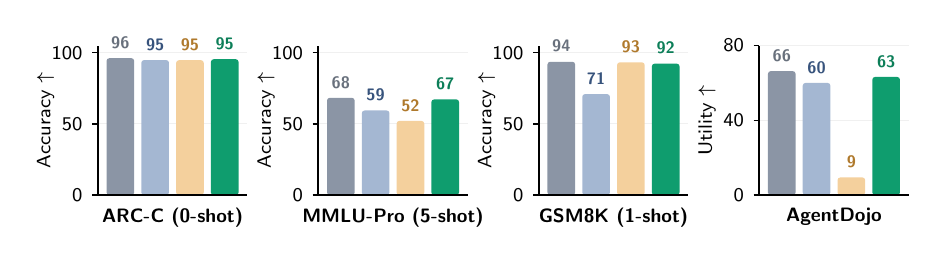
\begin{tikzpicture}[baseline=(axC.north)]
    \begin{axis}[teaser bars, name=axC, benchbelow={ARC-C (0-shot)},
      ylabel={Accuracy $\uparrow$},
      nodes near coords style={/pgf/number format/precision=0},
      ymin=0, ymax=105, ytick={0,50,100},
    ]
      % paper Table 2, 0-shot
      \addplot[bbar=cbase]  coordinates {(1,96.1)};
      \addplot[mbar=csec]   coordinates {(2,94.8)};
      \addplot[mbar=caside] coordinates {(3,94.7)};
      \addplot[obar=cours]  coordinates {(4,95.4)};
    \end{axis}
    \begin{axis}[teaser bars, name=axA, benchbelow={MMLU-Pro (5-shot)},
      at={($(axC.north east)+(9mm,0)$)}, anchor=north west,
      ylabel={Accuracy $\uparrow$},
      nodes near coords style={/pgf/number format/precision=0},
      ymin=0, ymax=105, ytick={0,50,100},
    ]
      % 5-shot
      \addplot[bbar=cbase]  coordinates {(1,68.3)};
      \addplot[mbar=csec]   coordinates {(2,59.4)};
      \addplot[mbar=caside] coordinates {(3,52.1)};
      \addplot[obar=cours]  coordinates {(4,67.2)};
    \end{axis}
    \begin{axis}[teaser bars, name=axG, benchbelow={GSM8K (1-shot)},
      at={($(axA.north east)+(9mm,0)$)}, anchor=north west,
      ylabel={Accuracy $\uparrow$},
      nodes near coords style={/pgf/number format/precision=0},
      ymin=0, ymax=105, ytick={0,50,100},
    ]
      % 1-shot, strict match
      \addplot[bbar=cbase]  coordinates {(1,93.6)};
      \addplot[mbar=csec]   coordinates {(2,70.9)};
      \addplot[mbar=caside] coordinates {(3,93.2)}; 
      \addplot[obar=cours]  coordinates {(4,92.3)};
    \end{axis}
    \begin{axis}[teaser bars, name=axB, benchbelow={AgentDojo},
      at={($(axG.north east)+(9mm,0)$)}, anchor=north west,
      ylabel={Utility $\uparrow$},
      nodes near coords style={/pgf/number format/precision=0},
      ymin=0, ymax=80, ytick={0,40,80},
    ]
      \addplot[bbar=cbase]  coordinates {(1,66.3)};
      \addplot[mbar=csec]   coordinates {(2,60.0)};
      \addplot[mbar=caside] coordinates {(3,9.47)}; % 9/95 clean tasks; plotted as 9.47 so the label rounds to 9, not 10
      \addplot[obar=cours]  coordinates {(4,63.2)};
    \end{axis}
\end{tikzpicture}%
}%
\sbox\secbox{%
% =============== SECURITY group ===============
  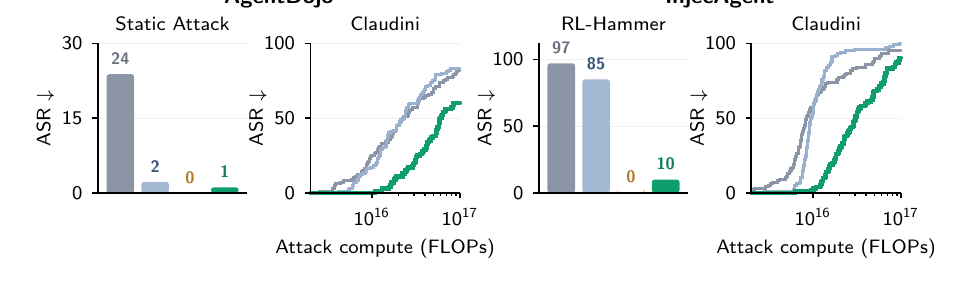
\begin{tikzpicture}[baseline=(adl.north)]
    % --- AgentDojo: static-attack bars + Claudini curve ---
    \begin{axis}[teaser bars, name=adl, subtitle={Static Attack},
      ylabel={ASR $\downarrow$},
      nodes near coords style={/pgf/number format/precision=0},% whole numbers, like the other bar panels
      ymin=0, ymax=30, ytick={0,15,30},
    ]
      \addplot[bbar=cbase]  coordinates {(1,23.8)};
      \addplot[mbar=csec]   coordinates {(2,2.2)};
      \addplot[mbar=caside] coordinates {(3,0.0)};
      \addplot[obar=cours]  coordinates {(4,1.1)};
    \end{axis}
    \begin{axis}[teaser curves, xmode=log, name=adr, subtitle={Claudini},
      at={($(adl.north east)+(8mm,0)$)}, anchor=north west,
      ylabel={ASR $\downarrow$},
      xlabel={Attack compute (FLOPs)}, xlabel style={yshift=2pt, font=\fsz{7}},
      xmin=2e15, xmax=1e17, xtick={1e16,1e17},
    ]
      % cumulative ASR against attack compute, as a step function
      \addplot[bline=cbase] coordinates {
        (2e+15,0) (2.52e+15,1) (3.56e+15,2) (3.6e+15,3) (3.73e+15,4) (3.77e+15,5) (3.9e+15,6) (4.43e+15,7)
        (4.75e+15,8) (5.91e+15,9) (6.12e+15,10) (6.56e+15,11) (6.79e+15,12) (7.62e+15,13) (7.71e+15,14) (7.8e+15,15)
        (8.17e+15,16) (8.66e+15,18) (8.76e+15,19) (8.86e+15,20) (9.17e+15,21) (9.28e+15,22) (9.38e+15,23) (9.72e+15,24)
        (9.94e+15,25) (1.08e+16,26) (1.09e+16,27) (1.16e+16,29) (1.18e+16,30) (1.22e+16,31) (1.28e+16,32) (1.3e+16,33)
        (1.41e+16,34) (1.56e+16,36) (1.63e+16,37) (1.65e+16,38) (1.73e+16,40) (1.77e+16,41) (1.85e+16,42) (1.88e+16,43)
        (1.9e+16,45) (2.01e+16,46) (2.06e+16,47) (2.13e+16,48) (2.18e+16,49) (2.23e+16,50) (2.31e+16,51) (2.56e+16,52)
        (2.59e+16,53) (2.62e+16,54) (2.65e+16,55) (2.71e+16,56) (2.88e+16,57) (3.26e+16,59) (3.3e+16,60) (3.34e+16,61)
        (3.42e+16,62) (3.5e+16,63) (3.88e+16,64) (4.11e+16,65) (4.36e+16,66) (4.78e+16,67) (4.95e+16,68) (5e+16,69)
        (5.06e+16,70) (5.24e+16,71) (5.81e+16,72) (5.88e+16,74) (6.52e+16,75) (6.83e+16,76) (7.24e+16,77) (8.31e+16,78)
        (8.41e+16,79) (8.81e+16,80) (9.12e+16,81) (9.44e+16,82) (1e+17,82)};
      \addplot[mline=csec] coordinates {
        (2e+15,0) (4.23e+15,1) (5.46e+15,2) (5.52e+15,3) (5.98e+15,4) (6.05e+15,5) (6.12e+15,7) (6.64e+15,8)
        (6.95e+15,9) (7.03e+15,10) (7.11e+15,11) (7.36e+15,12) (7.89e+15,13) (8.36e+15,14) (8.76e+15,16) (9.6e+15,17)
        (1.03e+16,18) (1.09e+16,19) (1.13e+16,20) (1.16e+16,21) (1.17e+16,23) (1.2e+16,24) (1.21e+16,25) (1.24e+16,27)
        (1.25e+16,29) (1.31e+16,30) (1.42e+16,31) (1.46e+16,34) (1.47e+16,35) (1.49e+16,38) (1.54e+16,40) (1.61e+16,41)
        (1.77e+16,42) (1.9e+16,44) (1.92e+16,45) (2.06e+16,47) (2.08e+16,48) (2.13e+16,49) (2.26e+16,50) (2.34e+16,51)
        (2.39e+16,52) (2.42e+16,55) (2.47e+16,57) (2.59e+16,58) (2.62e+16,59) (2.68e+16,60) (3.26e+16,62) (3.38e+16,63)
        (3.5e+16,64) (3.54e+16,65) (3.58e+16,66) (3.75e+16,67) (3.88e+16,68) (3.97e+16,69) (4.06e+16,70) (4.11e+16,71)
        (4.31e+16,72) (4.61e+16,73) (4.67e+16,74) (4.83e+16,75) (5.12e+16,76) (5.24e+16,77) (5.3e+16,79) (6.23e+16,80)
        (7.07e+16,81) (7.49e+16,82) (7.76e+16,83) (1e+17,83)};
      \addplot[oline=cours] coordinates {
        (2e+15,0) (1.08e+16,1) (1.3e+16,2) (1.31e+16,3) (1.56e+16,4) (1.63e+16,5) (1.65e+16,6) (1.67e+16,7)
        (1.77e+16,8) (1.79e+16,9) (1.85e+16,10) (1.9e+16,11) (2.23e+16,13) (2.39e+16,14) (2.42e+16,15) (2.5e+16,16)
        (2.56e+16,17) (2.88e+16,18) (2.94e+16,19) (3.01e+16,20) (3.08e+16,21) (3.12e+16,22) (3.15e+16,24) (3.26e+16,25)
        (3.54e+16,26) (3.71e+16,27) (3.75e+16,28) (3.93e+16,29) (4.11e+16,30) (4.16e+16,31) (4.21e+16,33) (4.26e+16,34)
        (4.46e+16,35) (4.61e+16,36) (4.72e+16,37) (4.95e+16,38) (5.36e+16,40) (5.42e+16,42) (5.49e+16,43) (5.55e+16,44)
        (5.81e+16,47) (5.88e+16,49) (5.95e+16,50) (6.16e+16,51) (6.3e+16,52) (6.38e+16,54) (6.75e+16,55) (6.83e+16,56)
        (7.94e+16,57) (8.31e+16,59) (8.41e+16,60) (1e+17,60)};
    \end{axis}
    % --- InjecAgent: RL-Hammer bars + Claudini curve ---
    \begin{axis}[teaser bars, name=inl, subtitle={RL-Hammer},
      at={($(adr.north east)+(10mm,0)$)}, anchor=north west,
      ylabel={ASR $\downarrow$},
      ymin=0, ymax=112, ytick={0,50,100},
      nodes near coords style={/pgf/number format/fixed, /pgf/number format/precision=0},
    ]
      % strongest of three RL-Hammer attackers per target, mean over five attack sets
      \addplot[bbar=cbase]  coordinates {(1,97)};
      \addplot[mbar=csec]   coordinates {(2,85)};
      \addplot[pbar=caside] coordinates {(3,0)}; 
      \addplot[obar=cours]  coordinates {(4,10)};
    \end{axis}
    \begin{axis}[teaser curves, xmode=log, name=inr, subtitle={Claudini},
      at={($(inl.north east)+(8mm,0)$)}, anchor=north west,
      ylabel={ASR $\downarrow$},
      xlabel={Attack compute (FLOPs)}, xlabel style={yshift=2pt, font=\fsz{7}},
      xmin=2e15, xmax=1e17, xtick={1e16,1e17},
    ]
      % cumulative ASR against attack compute, as a step function
      \addplot[bline=cbase] coordinates {
        (2e+15,2) (2.17e+15,3) (2.93e+15,4) (3.17e+15,5) (3.28e+15,6) (3.52e+15,7) (3.99e+15,8) (4.18e+15,9)
        (4.92e+15,10) (5.03e+15,11) (5.15e+15,13) (5.39e+15,14) (5.58e+15,15) (5.65e+15,16) (5.85e+15,17) (6.05e+15,19)
        (6.12e+15,22) (6.34e+15,23) (6.41e+15,24) (6.56e+15,26) (6.79e+15,29) (6.95e+15,30) (7.11e+15,31) (7.2e+15,32)
        (7.28e+15,35) (7.36e+15,38) (7.45e+15,39) (7.62e+15,40) (7.71e+15,41) (7.8e+15,43) (7.98e+15,45) (8.17e+15,48)
        (8.27e+15,49) (8.46e+15,51) (8.66e+15,52) (8.96e+15,54) (9.07e+15,55) (9.28e+15,56) (9.38e+15,57) (1.01e+16,59)
        (1.02e+16,60) (1.04e+16,61) (1.07e+16,63) (1.09e+16,65) (1.14e+16,66) (1.17e+16,67) (1.22e+16,68) (1.24e+16,69)
        (1.33e+16,70) (1.34e+16,71) (1.39e+16,73) (1.47e+16,74) (1.88e+16,76) (1.96e+16,77) (2.2e+16,78) (2.28e+16,79)
        (2.39e+16,80) (2.65e+16,81) (2.68e+16,82) (2.84e+16,83) (3.15e+16,84) (3.97e+16,86) (4.72e+16,87) (4.89e+16,88)
        (5e+16,89) (5.06e+16,90) (5.75e+16,91) (5.88e+16,92) (6.02e+16,93) (7.24e+16,94) (7.32e+16,95) (1e+17,95)};
      \addplot[mline=csec] coordinates {
        (2e+15,0) (2.79e+15,1) (6.05e+15,2) (6.12e+15,4) (6.19e+15,5) (6.49e+15,6) (7.03e+15,7) (7.2e+15,9)
        (7.28e+15,10) (7.54e+15,11) (7.62e+15,13) (7.71e+15,15) (7.8e+15,16) (7.89e+15,18) (7.98e+15,22) (8.17e+15,24)
        (8.36e+15,25) (8.46e+15,27) (8.56e+15,30) (8.66e+15,33) (8.76e+15,35) (8.86e+15,37) (8.96e+15,40) (9.07e+15,43)
        (9.17e+15,46) (9.28e+15,47) (9.38e+15,48) (9.49e+15,50) (9.72e+15,51) (9.94e+15,53) (1.01e+16,55) (1.02e+16,56)
        (1.03e+16,59) (1.04e+16,61) (1.05e+16,62) (1.09e+16,63) (1.1e+16,66) (1.14e+16,68) (1.16e+16,69) (1.18e+16,70)
        (1.2e+16,71) (1.21e+16,72) (1.24e+16,74) (1.27e+16,76) (1.31e+16,78) (1.36e+16,80) (1.37e+16,82) (1.42e+16,84)
        (1.51e+16,85) (1.56e+16,86) (1.58e+16,87) (1.61e+16,88) (1.65e+16,91) (1.79e+16,92) (1.9e+16,93) (2.06e+16,94)
        (2.34e+16,95) (2.98e+16,96) (6.75e+16,97) (7.49e+16,98) (8.22e+16,99) (9.66e+16,100) (1e+17,100)};
      \addplot[oline=cours] coordinates {
        (2e+15,0) (6.27e+15,1) (9.6e+15,2) (1.02e+16,3) (1.08e+16,4) (1.2e+16,5) (1.24e+16,6) (1.25e+16,7)
        (1.27e+16,8) (1.31e+16,10) (1.37e+16,11) (1.39e+16,12) (1.41e+16,14) (1.49e+16,15) (1.51e+16,16) (1.52e+16,17)
        (1.54e+16,18) (1.56e+16,19) (1.67e+16,20) (1.73e+16,21) (1.77e+16,22) (1.79e+16,23) (1.83e+16,26) (1.94e+16,27)
        (1.96e+16,28) (1.99e+16,29) (2.01e+16,30) (2.06e+16,31) (2.13e+16,32) (2.15e+16,33) (2.26e+16,36) (2.28e+16,37)
        (2.31e+16,38) (2.45e+16,39) (2.47e+16,40) (2.53e+16,41) (2.62e+16,42) (2.65e+16,43) (2.71e+16,44) (2.84e+16,45)
        (2.91e+16,47) (2.94e+16,48) (3.01e+16,49) (3.05e+16,51) (3.15e+16,53) (3.19e+16,54) (3.26e+16,55) (3.3e+16,56)
        (3.38e+16,57) (3.5e+16,58) (3.93e+16,59) (3.97e+16,60) (4.16e+16,61) (4.56e+16,62) (4.78e+16,64) (4.89e+16,67)
        (4.95e+16,68) (5.36e+16,69) (5.62e+16,70) (5.68e+16,71) (5.95e+16,72) (6.02e+16,73) (6.38e+16,74) (6.45e+16,75)
        (6.52e+16,77) (6.6e+16,78) (6.68e+16,80) (6.91e+16,81) (6.99e+16,83) (8.12e+16,84) (8.61e+16,86) (8.81e+16,87)
        (9.44e+16,88) (9.55e+16,89) (9.66e+16,90) (1e+17,90)};
    \end{axis}
    \benchhdr{($(inl.north)!0.5!(inr.north)$)}{InjecAgent}
    \benchhdr{($(adl.north)!0.5!(adr.north)$)}{AgentDojo}
  \end{tikzpicture}

}%
% card content as in the paper: title strut, then the plots
\sbox\ucontent{\begin{tabular}{@{}c@{}}\rule{0pt}{9mm}\\[-2mm]\usebox\utilbox\end{tabular}}%
\sbox\scontent{\begin{tabular}{@{}c@{}}\rule{0pt}{9mm}\\[-2mm]\usebox\secbox\end{tabular}}%
% both cards take the taller content's height (as in the paper) and the wider content's width (stacked)
\ifdim\dimexpr\ht\scontent+\dp\scontent\relax>\dimexpr\ht\ucontent+\dp\ucontent\relax
  \setlength\cardh{\dimexpr\ht\scontent+\dp\scontent+2\cardpad\relax}\else
  \setlength\cardh{\dimexpr\ht\ucontent+\dp\ucontent+2\cardpad\relax}\fi
\ifdim\wd\scontent>\wd\ucontent
  \setlength\cardw{\dimexpr\wd\scontent+2\cardpad\relax}\else
  \setlength\cardw{\dimexpr\wd\ucontent+2\cardpad\relax}\fi
\begin{minipage}{\cardw}
  \centering
  % ---- shared legend: the paper's one line, scaled down uniformly to the cards' width ----
  \resizebox{\cardw}{!}{\fsz{11.8}%
    \swatch{cbase}~GPT-OSS-20B\hspace{2em}%
    \swatch{csec!50}~w/ SecAlign\hspace{2em}%
    \swatch{caside!50}~w/ ASIDE\hspace{2em}%
    \swatch{cours}~w/ \textbf{H}eads \textbf{o}f \textbf{S}ecurity (ours)}

  \vspace{3mm}% gap between the legend and the chart cards
  % ---- two faint cards: utility (steel-blue tint) above security (vermilion tint), names in the corners ----
  
\begin{tikzpicture}
    \node[anchor=north west, inner sep=\cardpad, rounded corners=8pt, fill=tblue!6, draw=none, minimum width=\cardw, minimum height=\cardh] (uc) at (0,0) {\usebox\ucontent};
    \node[anchor=north west, inner sep=\cardpad, rounded corners=8pt, fill=tred!5, draw=none, minimum width=\cardw, minimum height=\cardh] (sc) at ($(uc.south west)+(0,-3mm)$) {\usebox\scontent};
    \node[anchor=north west, font=\robotolight\fsz{11.8}, text=black, inner sep=0pt] at ($(uc.north west)+(4mm,-3mm)$) {Utility};
    \node[anchor=north west, font=\robotolight\fsz{11.8}, text=black, inner sep=0pt] at ($(sc.north west)+(4mm,-3mm)$) {Security};
  \end{tikzpicture}
\end{minipage}
\end{document}
